\documentclass{amsart}

\setlength{\textwidth}{13cm}
\setlength{\textheight}{19cm}

\usepackage{graphicx} 		% balik pro vkladani obrazku
\usepackage{amsmath, amsthm, amssymb}
\usepackage{natbib}

%\usepackage[cp1250]{inputenc} 	% kodovani cestiny MS Windows
%\usepackage[latin2]{inputenc} 	% kodovani cestiny Linux
\usepackage[utf8]{inputenc}
\usepackage{comment}

\newtheorem{theorem}{Theorem}
\newtheorem{corollary}[theorem]{Corollary}
\theoremstyle{definition}\newtheorem{definition}[theorem]{Definition}
\theoremstyle{remark}\newtheorem{remark}[theorem]{Remark}

\newcommand{\dif}{\,\mathrm{d}}
\newcommand{\e}{\,\mathrm{e}}
\newcommand{\E}{\,\mathrm{E}}
\newcommand{\D}{\,\mathrm{D}}
\newcommand{\ds}{\,\mathrm{d}s}
\newcommand{\dt}{\,\mathrm{d}t}
\newcommand{\dW}{\,\mathrm{d}W}
\newcommand{\PR}{\,\mathrm{P}}

\begin{document}

\title{Credit Risk Modeling of Financial Derivatives}
\author{KAFKOVÁ Silvie and KŘIVÁNKOVÁ Lenka}

\begin{abstract}
\end{abstract}
\maketitle

\noindent\textbf{Keywords:} credit valuation adjustment, probability of default, interest rate swaps, Hull-White model, Monte Carlo simulations, credit exposure

\bigskip

\section{Introduction}
As a motivation to why one would need a risk measure to capture shifts in credit spread, the Basel Committee estimate that about three fourths of the CCR losses during the financial crisis originate from CVA losses and not actual defaults.

\section{Methods of credit valuation adjustment computation}
In this section, we developed the basic methodology to compute CVA and describe the basic terms.

\subsection{Components of credit valuation adjustment and terminology}
%přidat definici defaultu a zdůraznit, že veškeré úvahy počítají default v čase $t$. - asi není nutné
The basic concepts and notation for counterparty credit risk and CVA will be shown in this section.
Counterparty credit risk (CCR) is the risk that the counterparty defaults before the final settlement of a transaction's cash flows.
CVA can be explained as the difference between the portfolio’s risk-free value and the portfolio’s true value taking into account the possibility of default of the counterparty.
In the next definition CVA is calculated as expectation of credit loss.
\begin{definition}
 \textit{The credit valuation adjustment} is defined as
 \begin{equation}
 CVA=(1-R)\int_{0}^T \hat{e_d}(t)\dif PD(t),
 \label{CVA}
\end{equation}
  where $R$ is recovery rate, $\hat{e_d}(t)$ is the discounted expected exposure at time $t$ and $PD(t)$ is probability of default.
\end{definition}
%We can observe that CVA depends on the following components:
In what follows, we specify the components of CVA. 
Recovery rate is the value of unity less \textit{Loss given default (LGD)}, i.e. $R=1-~LGD$.
The LGD is the percentage amount of the exposure expected to be lost if the counterparty defaults.

The counterparty credit exposure $E(t)$ of the bank to a counterparty at time $t$ (hereafter simply exposure) is defined as the economic loss, incurred on all outstanding transactions with the counterparty if the counterparty defaults at $t$.
Denote the value of the $i$-th instrument in the portfolio at time $t$ by  $V_i(t)$. 
The value of the counterparty portfolio is given by 
\begin{equation}
V(t)=\sum_{i=1}^N V_i(t).
\end{equation}
When netting is not allowed, the exposure E(t) is given by
\begin{equation}
E(t)=\sum_{i=1}^N\max\{V_i(t),0\}.
\end{equation}
For a counterparty portfolio with a netting agreement, the exposure is
\begin{equation}
E(t)=\max\{V(t),0\}.
\end{equation}

Discounting is a financial mechanism in which a future value is being recalculated to the present value.
The discount factor, $D(t)$, is the factor by which a future cash flow must be multiplied in order to obtain the present value.
Consider the discount factor at time $t$% (for maturity $T$)
, defined as 
%nemělo by T být spíš doba defaultu?
\begin{equation}
D(t)=\frac{B_0}{B_t}=e^{-rt},
\end{equation}
where $r$ is risk-free rate of return and $B_t$ is the value of risk free asset at time $t$. 
%spojité diskontování se v praxi napoužívá, ale usnaňuje výpočty
Hence, the discounted expected exposure at time $t$ conditional on the counterparty default at time $t$ is given by 
\begin{equation}
\hat{e}_d(t)=\E[D(t) E(t)].
\end{equation}

Next component of the equation \eqref{CVA} is default probability $PD(t)$ which describes the creditworthiness of a counterparty. 
It provides an estimate of the likelihood that a borrower will be unable to meet its debt obligations.
There are many alternatives for estimating the probability of default.
The frequently used approach, taken by many banks, is to use external ratings agencies (such as S\&P, Fitch or Moody's) for estimating $PD$ from historical default experience.

\begin{table}
\caption{Resulting CVA}
\scalebox{1}{\begin{tabular}{|c |r|}
\hline
\textbf{Counterparty} &\textbf{CVA (in CZK)}\\ 
\hline
$\boldsymbol{1}$ &1 056 075.83  \\ 
$\boldsymbol{2}$&265 290.14  \\
$\boldsymbol{3}$&369.19 \\
$\boldsymbol{4}$& 1 045.54\\
$\boldsymbol{5}$&103 319.55 \\
\hline
\end{tabular}}
\end{table}

\begin{figure}[!htbp]
  \centering 
	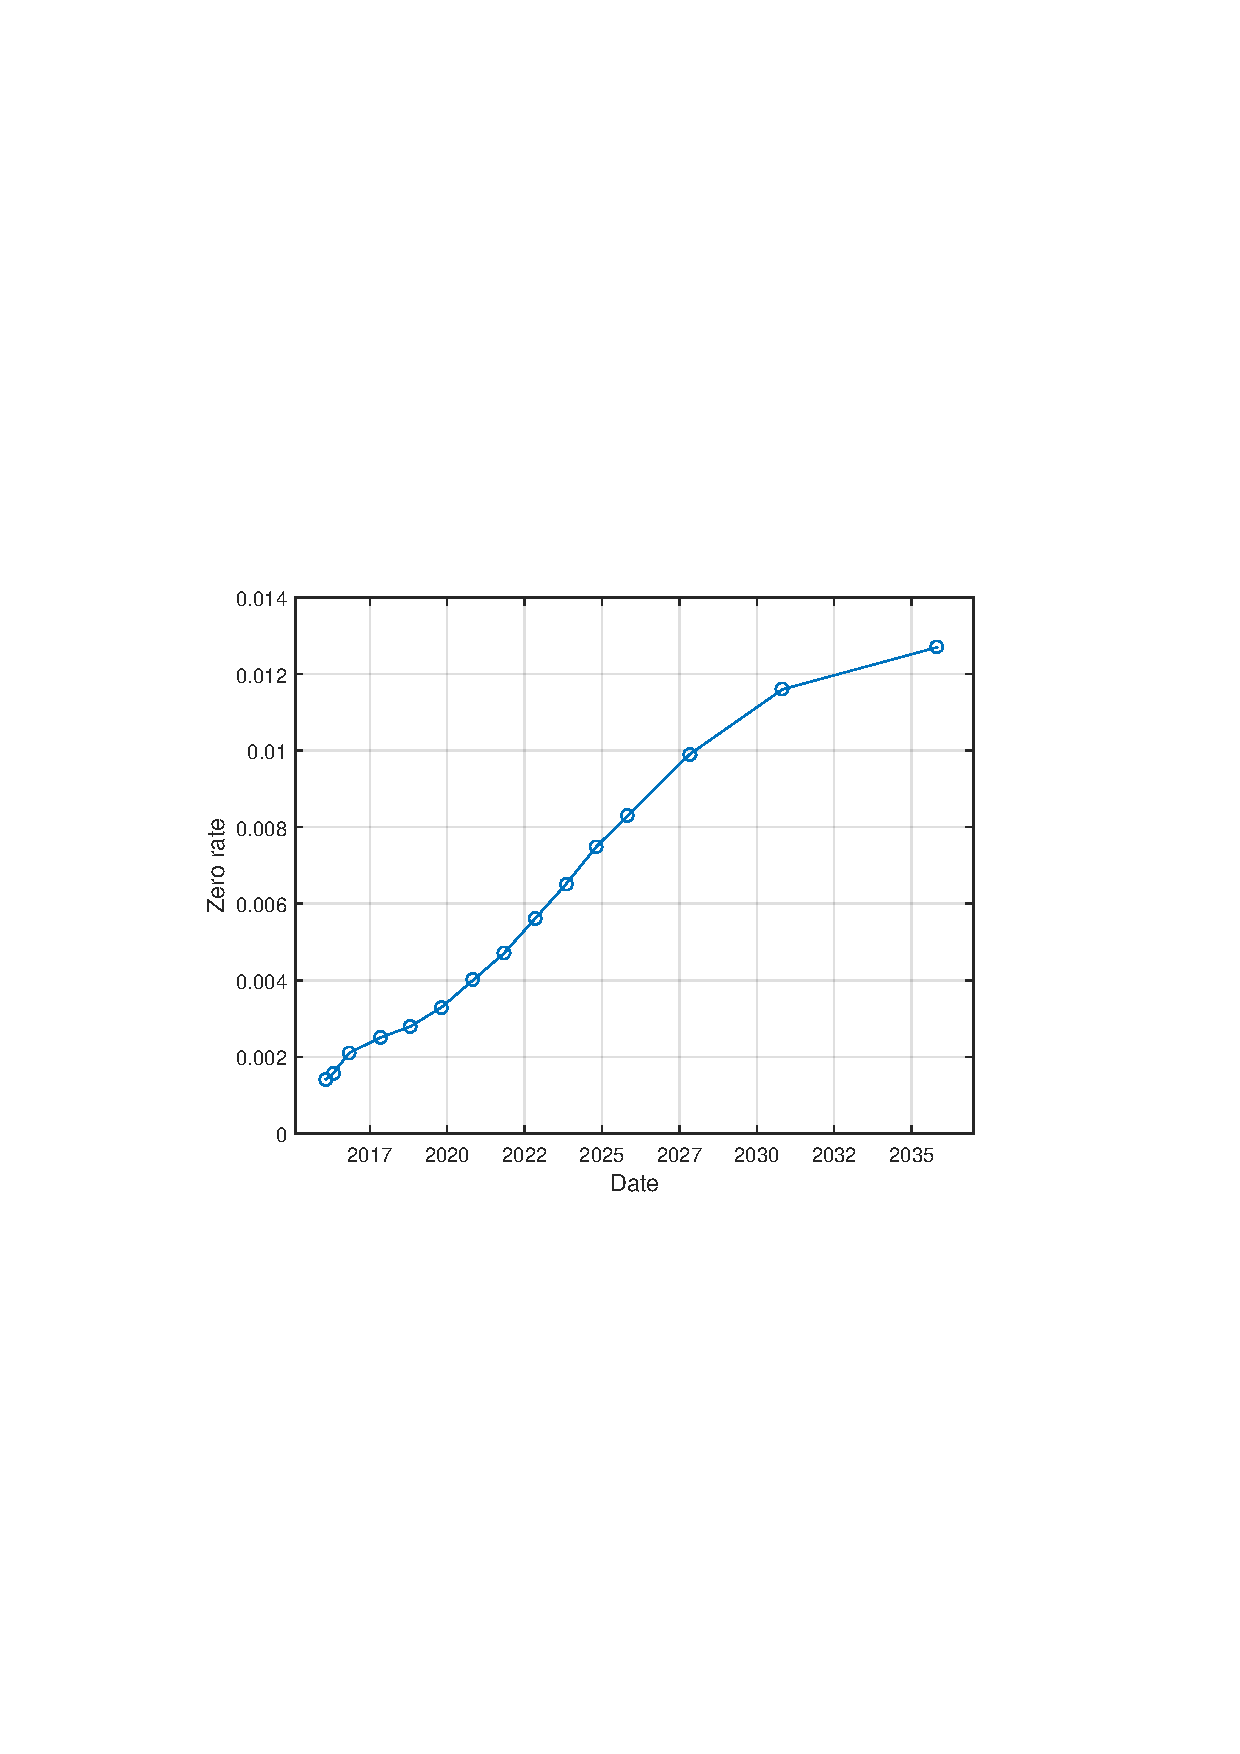
\includegraphics[width=6cm, clip, trim= 110 270 110 270]{IMG/YieldCurve.pdf}
  \caption{Yield Curve}  \label{YieldCurve}
\end{figure}

\begin{figure}[!htbp]
  \centering 
	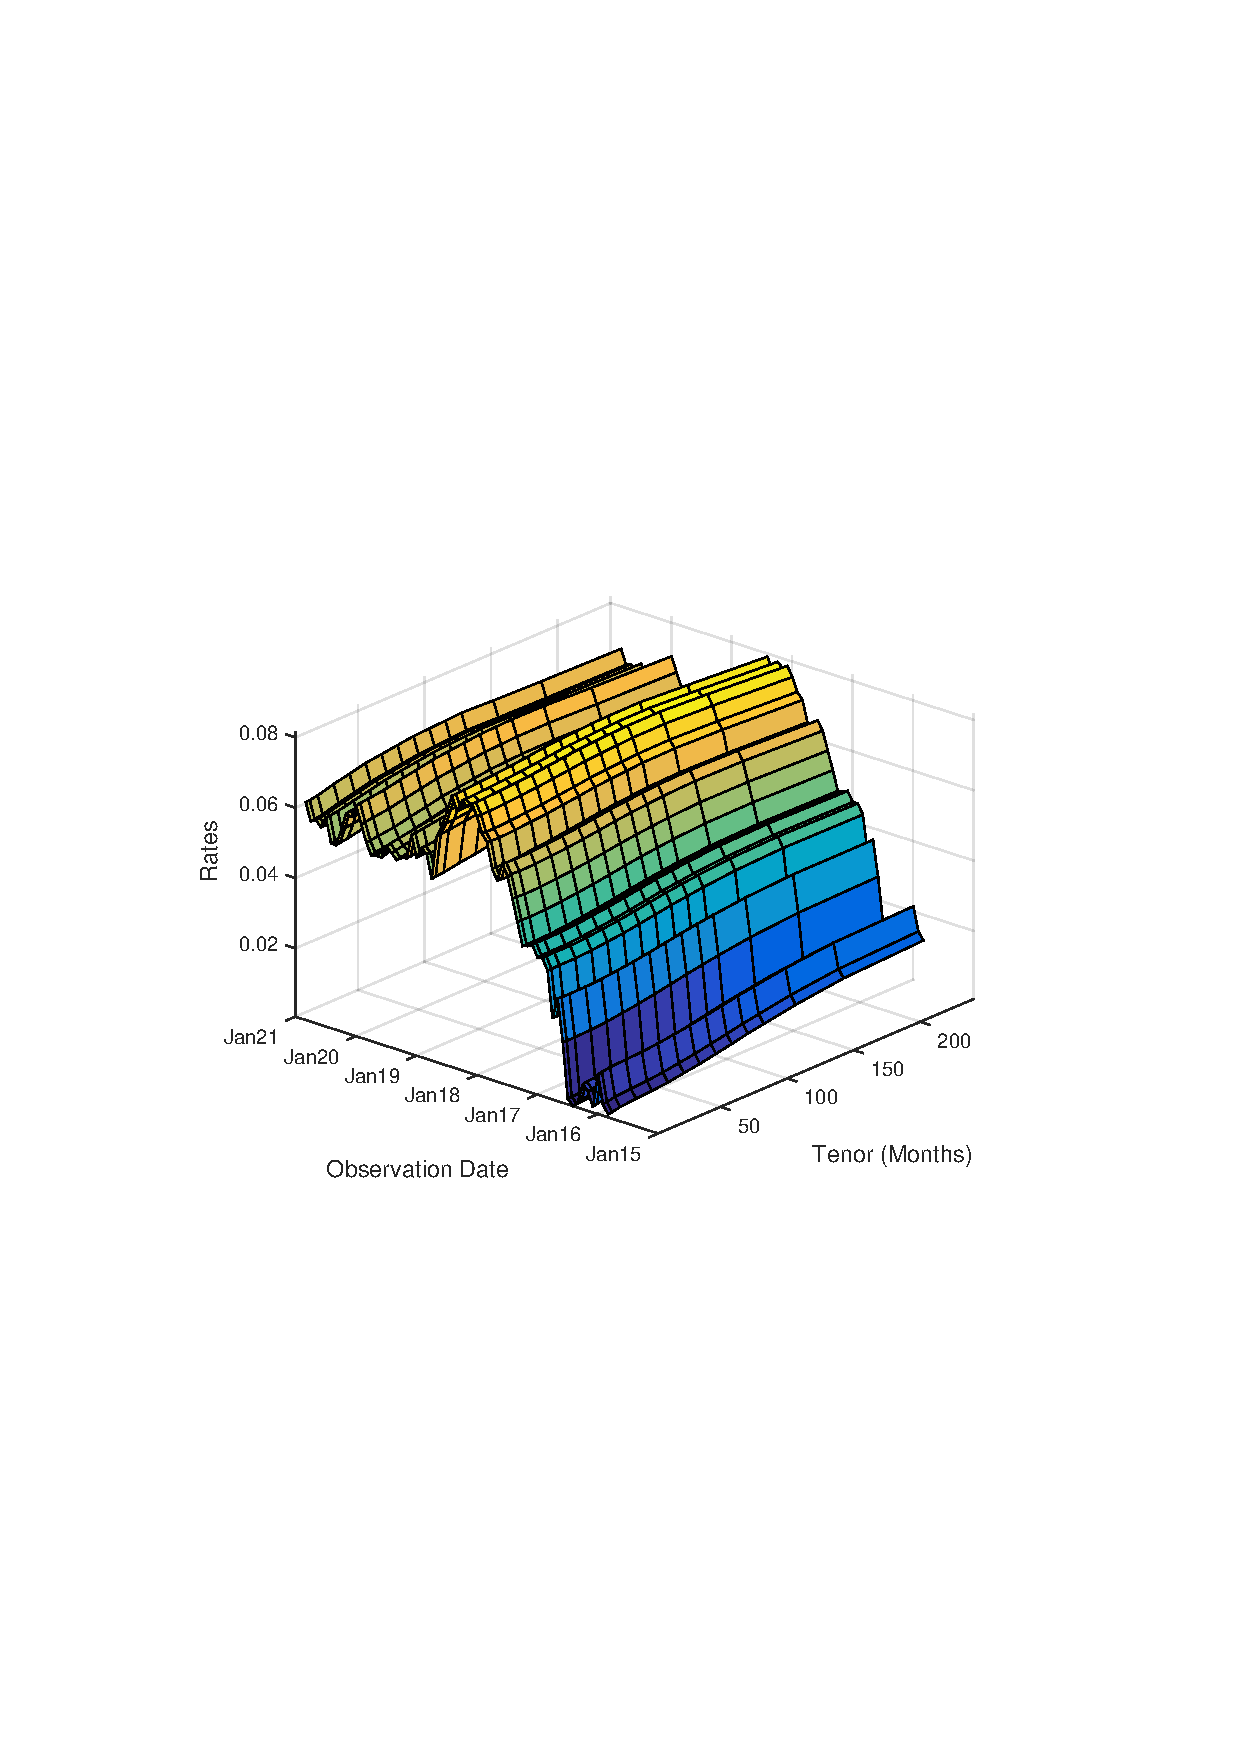
\includegraphics[width=6cm, clip, trim= 110 270 110 270]{IMG/YieldCurveEvolution.pdf}
  \caption{Yield Curve Evolution}  \label{YieldCurveEvolution}
\end{figure}

\begin{figure}[!htbp]
  \centering 
	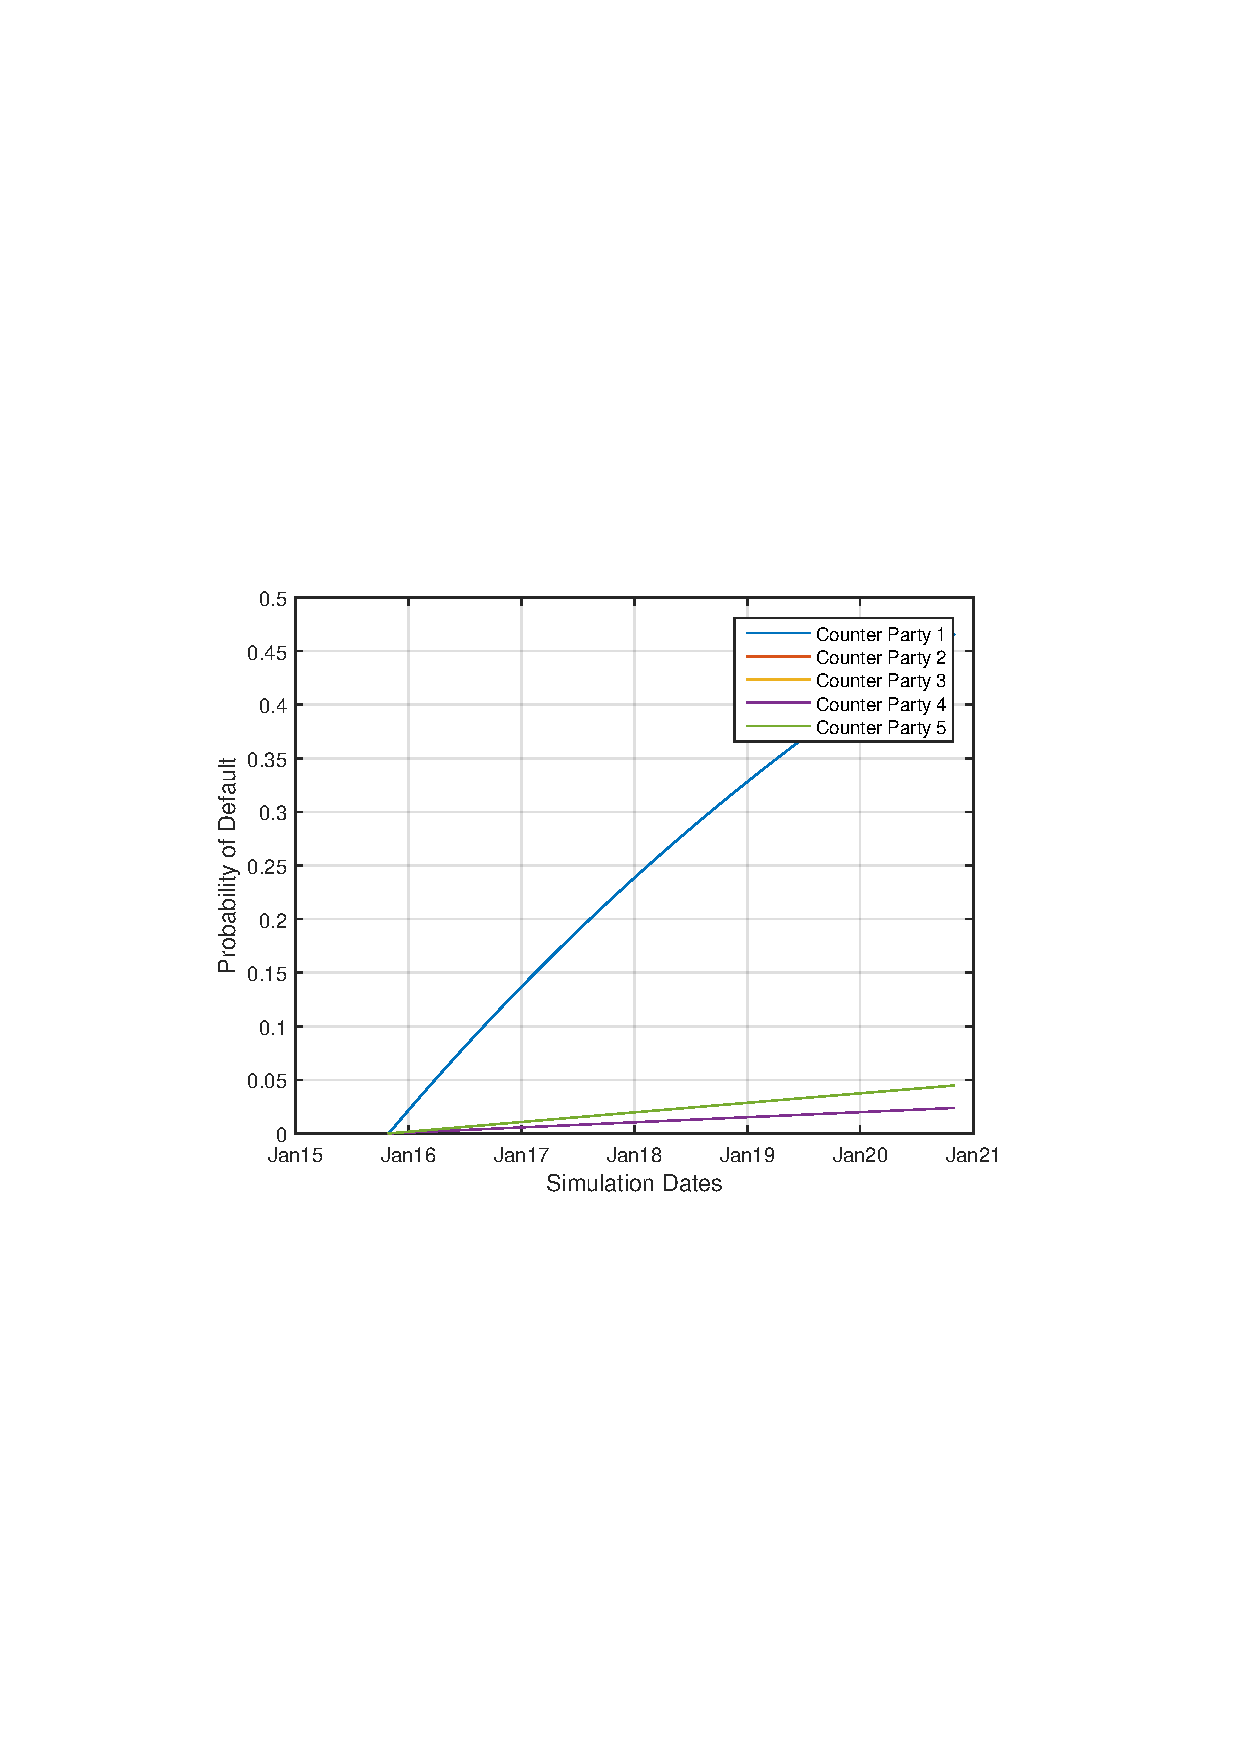
\includegraphics[width=6cm, clip, trim= 110 270 110 270]{IMG/DefaultProbability.pdf}
  \caption{Default Probability}  \label{DefaultProbability}
\end{figure}

\begin{figure}[!htbp]
  \centering 
	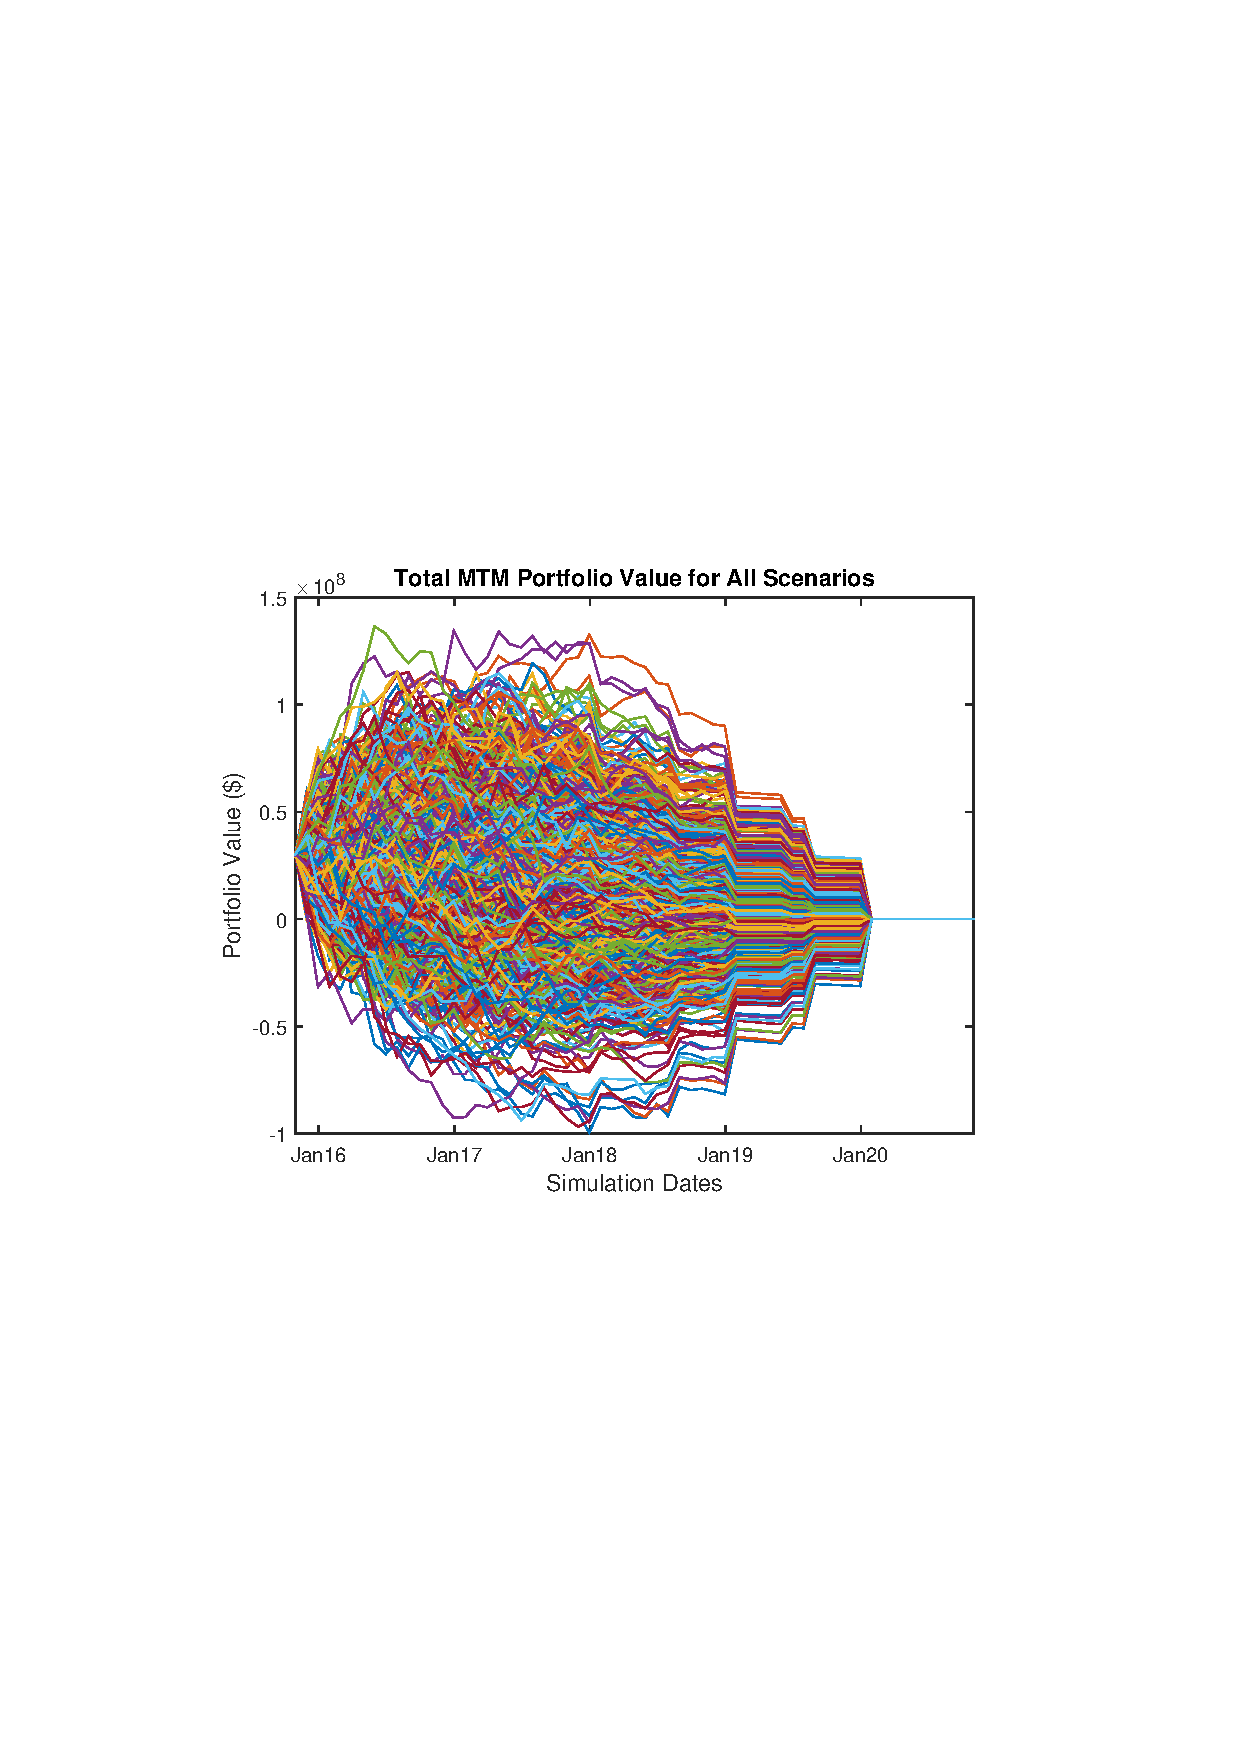
\includegraphics[width=6cm, clip, trim= 110 270 110 270]{IMG/TotalPortfoioValue.pdf}
  \caption{Total Portfoio Value}  \label{TotalPortfoioValue}
\end{figure}

\begin{figure}[!htbp]
  \centering 
	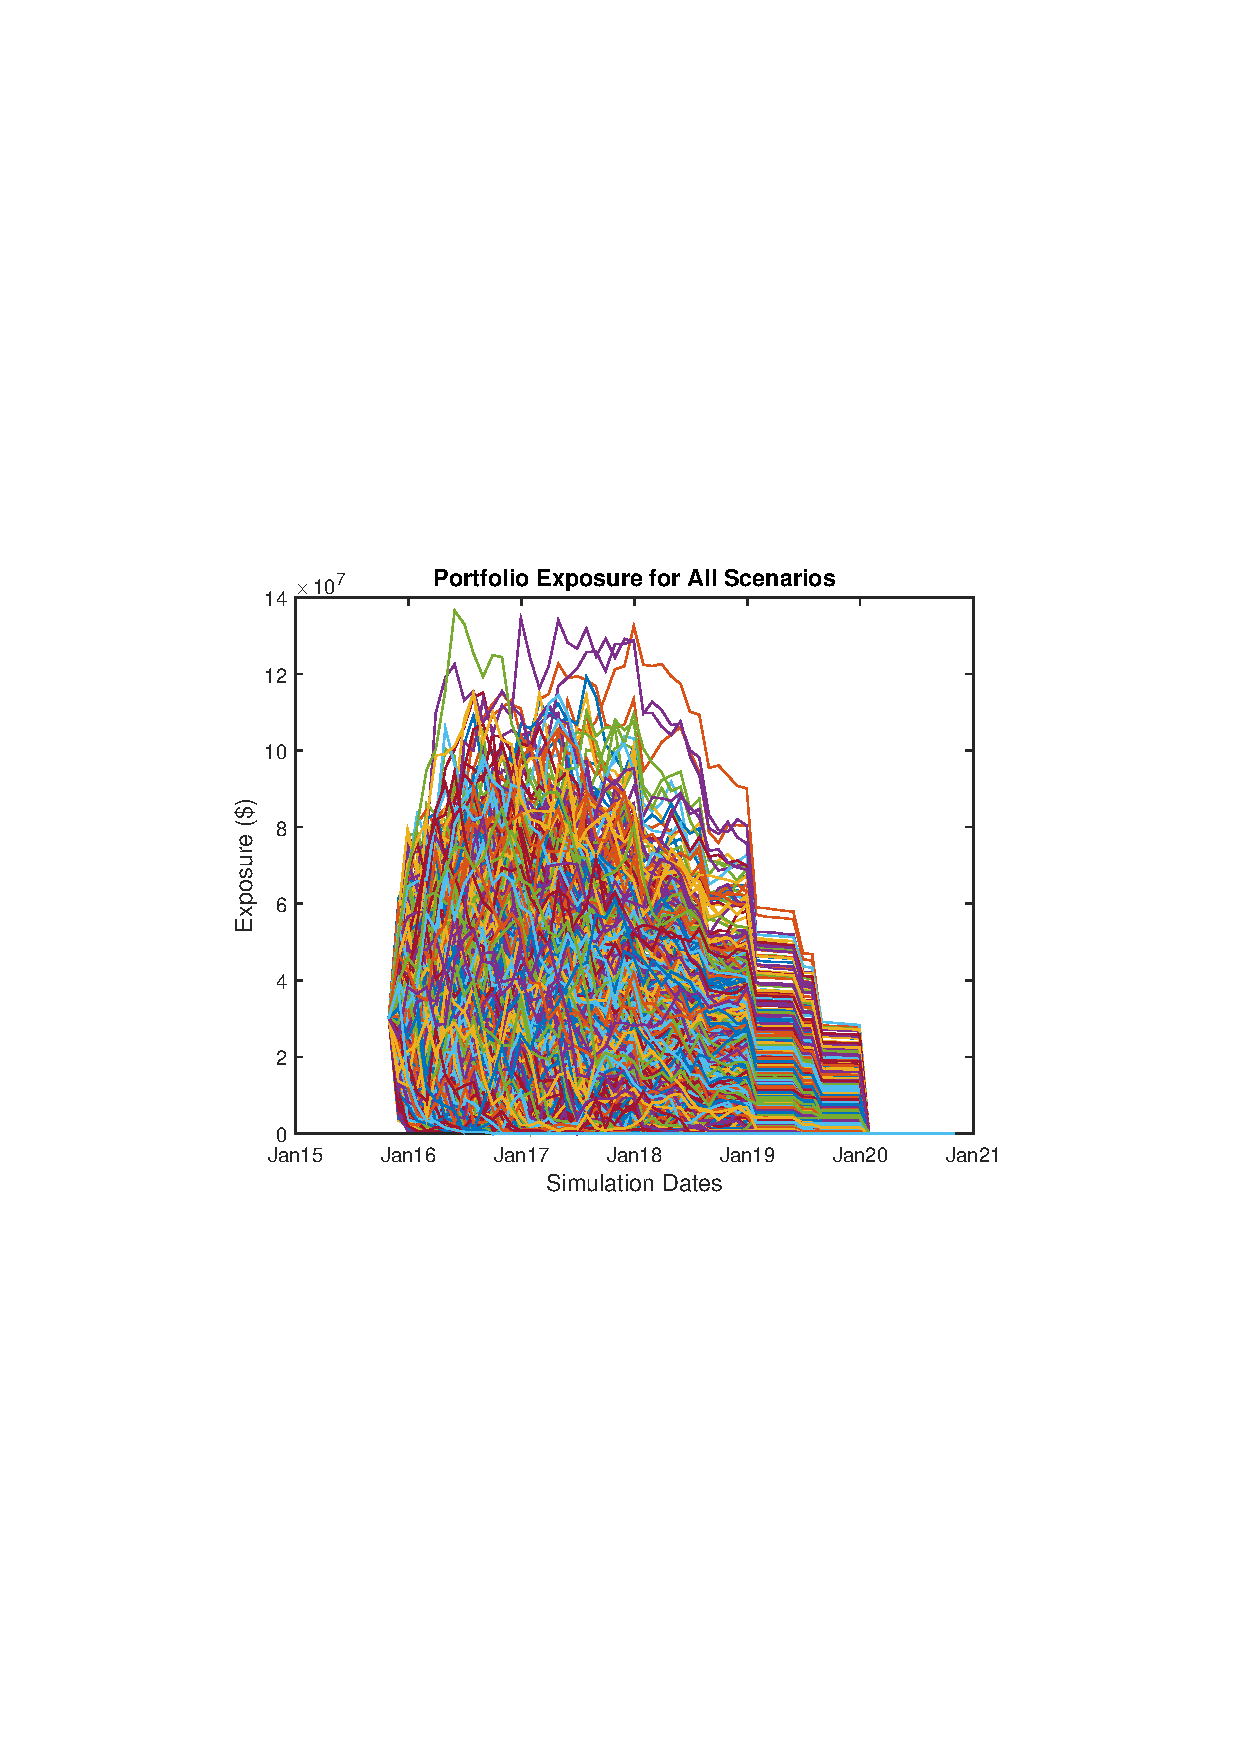
\includegraphics[width=6cm, clip, trim= 110 270 110 270]{IMG/PorfolioExposure.pdf}
  \caption{Porfolio Exposure}  \label{PorfolioExposure}
\end{figure}

\begin{figure}[!htbp]
  \centering 
	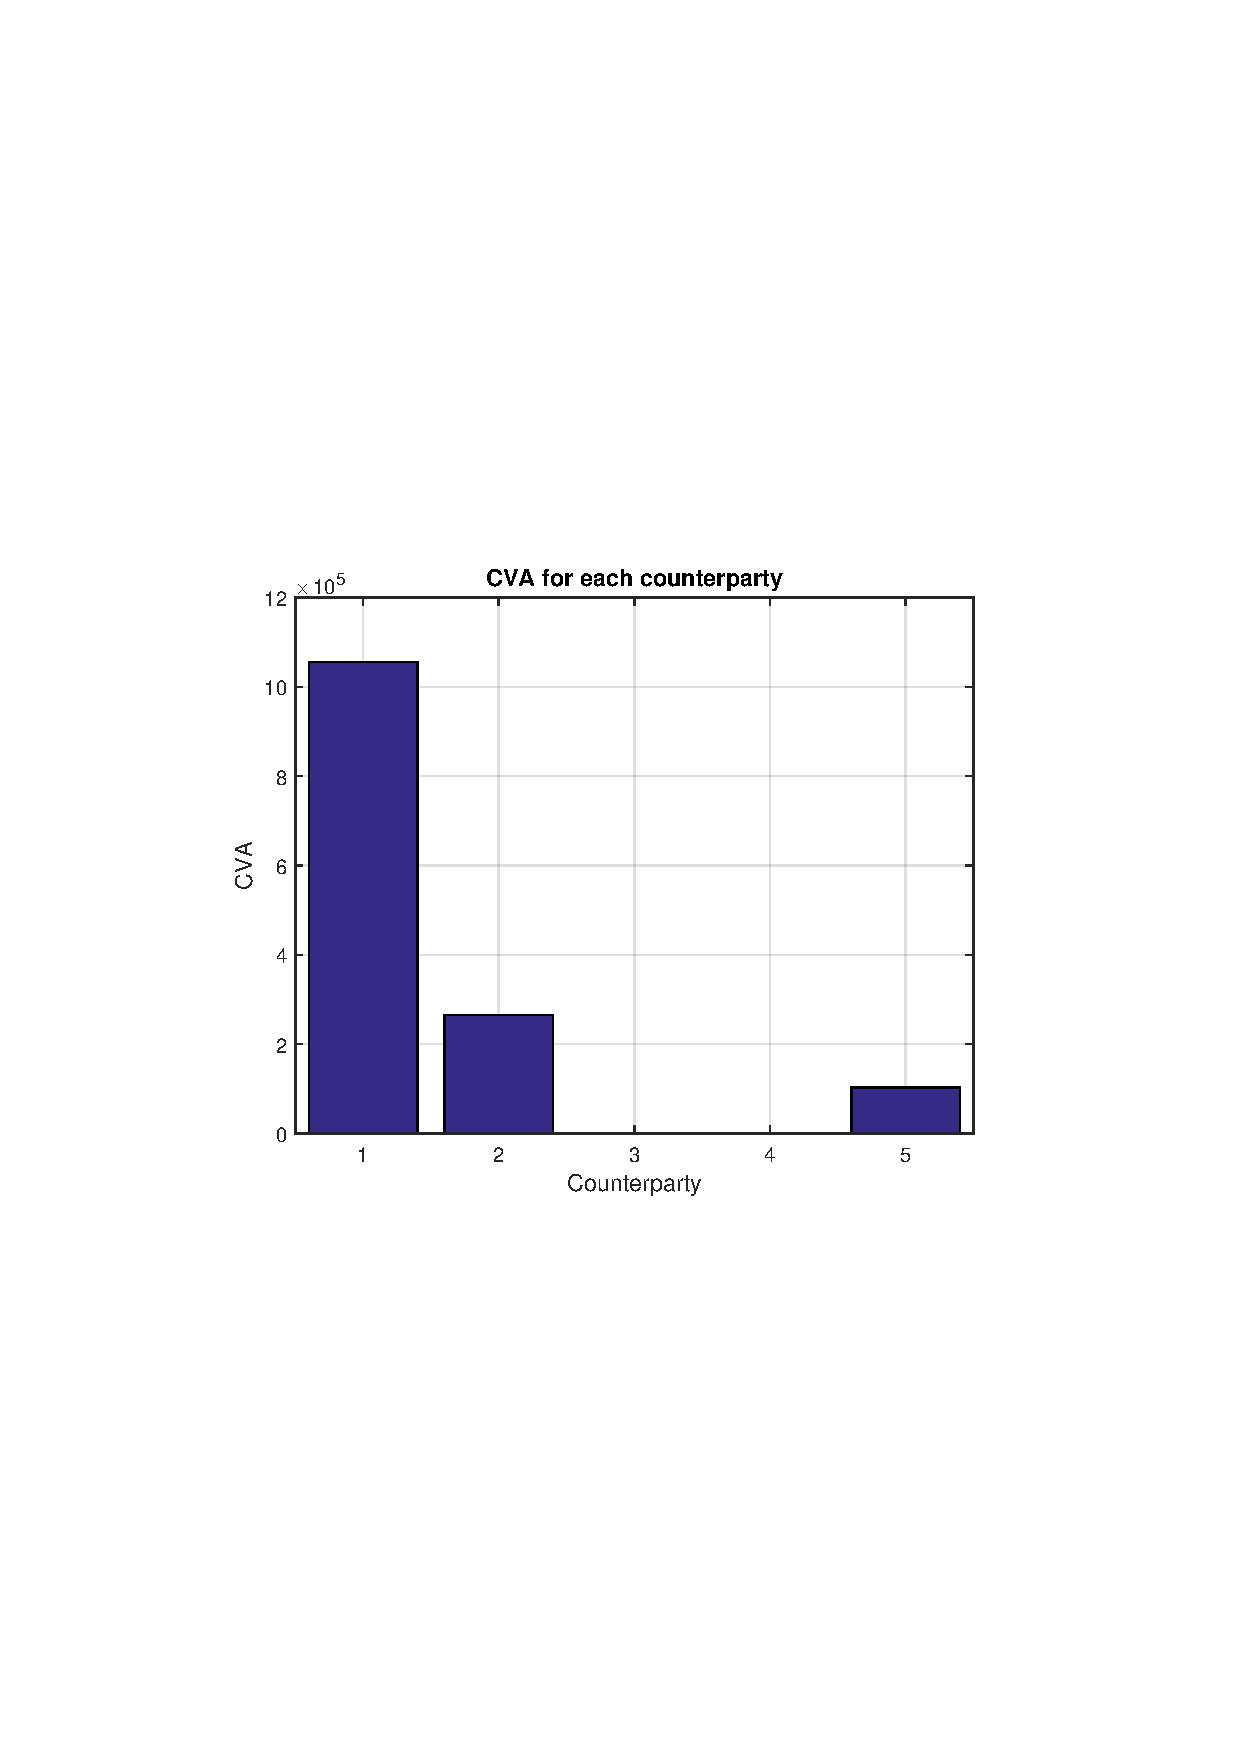
\includegraphics[width=6cm, clip, trim= 110 270 110 270]{IMG/CVAforEachCounterparty.pdf}
  \caption{CVA for each counterparty}  \label{CVAforEachCounterparty}
\end{figure}

%\section{Methods of Comparing Different Models}
%\subsection{Analysis of Deviance}
%\subsection{Information Criteria}
%\section{Applying Generalized Linear Models in Actuarial Science}

\begin{comment}
\begin{thebibliography}{99}
\bibitem[Antonio and Beirlant(2005)]{antonio}
ANTONIO Katrien, BEIRLANT Jan: Applications of generalized linear mixed models in actuarial statistics. {\it Insurance: Mathematics and Economics,} 2005.
\bibitem[Cerchiara, Edwards and Gambini(2008)]{rocco}
CERCHIARA Rocco Roberto, EDWARDS Matthew, GAMBINI Alessandra: Generalized linear models in life insurance: decrements and risk factor analysis under Solvency II. In: {\it 18th International AFIR Colloquium.} 2008.
\bibitem[Denuit(2007)]{denuit}
DENUIT Michel, et al.: {\it Actuarial modelling of claim counts: risk classification, credibility and bonus-malus systems.} Hoboken: Wiley. 2007.
\bibitem[Dobson(2002)]{dobson}
DOBSON Annette J.: {\it An Introduction to Generalized Linear Models.} Boca Raton: CRC Press. 2002.
\bibitem[Gschlössl, Schoenmaekers and Denuit(2011)]{gs}
GSCHLÖSSL Susanne, SCHOENMAEKERS Pascal, DENUIT Michel: Risk classification in life insurance: methodology and case study. {\it European Actuarial Journal,} 2011, 1.1: 23-41.
\bibitem[Haberman and Renshaw(1996)]{haberman}
HABERMAN, Steven; RENSHAW, Arthur E. Generalized linear models and actuarial science. {\it The Statistician,} 1996, 407-436.
\bibitem[Hardin and Hilbe(2007)]{hardin}
HARDIN James William, HILBE Joseph: {\it Generalized linear models and extensions.} Stata Corp, 2007.
\bibitem[Heller and Jong(2008)]{jong}
HELLER Gillian Z., JONG Piet: {\it Generalized Linear Models for Insurance Data.} New York: Cambridge University Press. 2008.
\bibitem[Kaas(2009)]{kaas}
KAAS Rob: {\it Modern Actuarial Risk Theory: Using R.} Heidelberg: Springer. 2009.
\bibitem[McCullagh and Nelder(1989)]{mc}
MCCULLAGH Peter, NELDER John A.: {\it Generalized Linear Models.} London: Chapman and Hall. 1989.
\bibitem[Nelder and Wedderburn(1972)]{nelder}
NELDER John A., WEDDERBURN Robert W. M.: Generalized linear models. {\it Journal of the Royal Statistical Society. Series A (General),} 1972, 370-384.
\bibitem[Ohlsson and Johansson(2010)]{ohlson}
OHLSSON Esbjörn, JOHANSSON Björn: {\it Non-life insurance pricing with generalized linear models.} Springer. 2010.
\bibitem[Wolny-Dominiak(2012)]{dominiak}
WOLNY-DOMINIAK Alicja: Modeling of claim counts using data mining procedures in R CRAN In: RAMÍK, J. and STAVÁREK, D. (eds.) 
{\it Proceedings of 30th International Conference Mathematical Methods in Economics.} Karviná: Silesian University, School of Business Administration, 2012, pp. 980-985.
\end{thebibliography}
\end{comment}

\nocite{bouchaud2003theory} 
\nocite{duffie2003intertemporal} 
\nocite{etheridge2002course} 
\nocite{hull} 
\nocite{pykhtin2010} 
\nocite{gregory2010} 
\nocite{brigo2014} 
\nocite{hull2012cva} 
\nocite{arora2012} 
\nocite{jilek2000} 
\nocite{canabarro2003measuring} 

\nocite{}  %umisti do literatury i necitovanou polozku a \nocite{*} umisti do literatury vsechny polozky z bibtex databaze 

%\bibliographystyle{plain}
\bibliographystyle{abbrv}
\bibliography{bibliography}

\end{document}